\documentclass[12pt,letterpaper]{article}
\usepackage{amsmath} % Paquete de ecuaciones
\usepackage{amsfonts}
\usepackage{amssymb}
\usepackage{graphicx} % Paquete de imágenes

\usepackage{subfigure} % Subfiguras
\usepackage{geometry}
\usepackage{float}
\usepackage[utf8]{inputenc} % Acentos y eñes
\usepackage{setspace} % Interlineado
\geometry{left=4cm, right=3cm, top=3cm, bottom=3cm} % Márgenes
\usepackage[spanish,es-tabla]{babel} % Tablas
\expandafter\def\csname ver@subfig.sty\endcsname{} 
\pagestyle{plain} 
\pagenumbering{arabic}
\usepackage{multicol} % Para varias columnas
\usepackage{subfig}
\bibliographystyle{plain} % Bibliografía
\usepackage{multirow}
\usepackage[hidelinks]{hyperref} % Links
\usepackage[usenames]{color} % Color para las palabras
\usepackage{textcomp}
\usepackage{enumitem}
\usepackage{pdfpages} % Para incluir PDF
\usepackage{multimedia}
\usepackage[document]{ragged2e}
\usepackage{times} % Tipo de letra Times
\spacing{1.5} % Interlineado

    \title{\normalsize \textbf{ENTRENAMIENTO INDUSTRIAL}\\
	{
	\\(PASANTÍA INDUSTRIAL)
	\\ 
	\\  
	\\
	\vspace*{1.0in}
	\large Título del trabajo
	\\
	\vspace{0.25in}
	\LARGE \textbf{}}
	\vspace*{1.0in}}

    \author{
     \\ \hspace{4in} \normalsize INFORME DE PASANTÍA  
     \\ \hspace{4in} \normalsize BR. ENDERSON OMAÑA   
     \\ \hspace{4in} \normalsize ESCUELA DE INGENIERÍA ELÉCTRICA    
     \\ \hspace{4in} \normalsize FACULTAD DE INGENIERÍA   
     \\ \hspace{3in} \normalsize UNIVERSIDAD CENTRAL DE VENEZUELA    
    \vspace*{1.5in}} % title llega hasta acá

    \date{\normalsize 31/07/19}

\begin{document}
%%%%%%%%%%%%%%%%%%%%%%%%%%%%%%%%%%%%
%%%%%%
%%%%%%          Portada
%%%%%%
%%%%%%%%%%%%%%%%%%%%%%%%%%%%%%%%%%%
    \thispagestyle{empty} 
\begin{center}
    \textbf{ENTRENAMIENTO INDUSTRIAL}\\
    (PASANTÍA INDUSTRIAL)\\

    \vspace{5cm}
    Título del trabajo
\end{center}    
    \vspace{5cm}
    \hspace{6cm}INFORME DE PASANTÍA\\
    \hspace{6cm}Br. Enderson Omaña\\
    \hspace{6cm}ESCUELA DE ELÉCTRICA\\
    \hspace{6cm}FACULTAD DE INGENIERÍA\\
    \hspace{6cm}UNIVERSIDAD CENTRAL DE VENEZUELA\\
    \vspace{5cm}
    \begin{center}
        Caracas, septiembre 2019
    \end{center}
%%%%%%%%%%%%%%%%%%%%%%%%%%%%%%%%%%%%
%%%%%%
%%%%%%         Contra portada
%%%%%%
%%%%%%%%%%%%%%%%%%%%%%%%%%%%%%%%%%%
    
\begin{center}
    \textbf{ENTRENAMIENTO INDUSTRIAL}\\
    (PASANTÍA INDUSTRIAL)\\

    \vspace{6cm}
    Diseño de interfaz de un SCADA para el monitoreo del 
    energético de un edificio residencial
\end{center}    
    \vspace{6cm}
    \hspace{6cm}TUTOR ACADEMICO: Ing. Güette Luis\\
    \hspace{6cm}TUTOR INDUSTRIAL: Prof. Panayotis Tremante\\

    \vspace{4cm}
    \begin{center}
        Caracas, septiembre 2019
    \end{center}
    \thispagestyle{empty} 
    \newpage 
%%%%%%%%%%%%%%%%%%%%%%%%%%%%%%%%%%%%
%%%%%%
%%%%%%         Resumen
%%%%%%
%%%%%%%%%%%%%%%%%%%%%%%%%%%%%%%%%%%
    \begin{center}
    \section*{RESUMEN} % El símbolo * no enumera la sección en el índice
    \thispagestyle{empty}
\end{center}

\newpage
%%%%%%%%%%%%%%%%%%%%%%%%%%%%%%%%%%%%
%%%%%%
%%%%%%         Índice
%%%%%%
%%%%%%%%%%%%%%%%%%%%%%%%%%%%%%%%%%%
    \begin{center}
        \tableofcontents    
    \end{center}
    \thispagestyle{empty}
    \newpage
%%%%%%%%%%%%%%%%%%%%%%%%%%%%%%%%%%%%
%%%%%%
%%%%%%         NOMENCLATURA, ABREVIATURA Y SÍMBOLOS   
%%%%%%
%%%%%%%%%%%%%%%%%%%%%%%%%%%%%%%%%%%
    \begin{center}
    \section*{NOMENCLATURA, ABREVIATURA Y SÍMBOLOS}
    \thispagestyle{empty}
\end{center}
\justify

\begin{list}{}{}

    \subsection*{LISTA DE ABREVIATURAS:}
    
        \item \textbf{SCADA:} Supervisory Control And Data Acquisition.
        \item \textbf{LAN:}  Local Area Network.
        \item \textbf{WAN:}  Wide Area Network.
        \item \textbf{IoT:} Internet of Things.
        \item \textbf{IIoT:} Industrial Internet of Things.
        \item \textbf{PLC:} Programmable Logic Controller.
        \item \textbf{API:} Application Programming Interface.
        \item \textbf{MangoES:} Mango Enterprise.
    
    \subsection*{LISTA DE SÍMBOLOS:}
    
        \item \textbf{V:} Volts.
        \item \textbf{A:} Ampere.
        \item \textbf{W:} Watts.
        \item \textbf{$\Omega$:} Ohms.
    
    \end{list}

\newpage
%%%%%%%%%%%%%%%%%%%%%%%%%%%%%%%%%%%%
%%%%%%
%%%%%%         INTRODUCCIÓN
%%%%%%
%%%%%%%%%%%%%%%%%%%%%%%%%%%%%%%%%%%   
    \setcounter{page}{1} % Para empezar a enumerar desde esta página
\begin{center}
    \section*{INTRODUCCIÓN}
\end{center}
\addcontentsline{toc}{section}{INTRODUCCIÓN} % Para incluir INTRODUCCIÓN en el índice

\newpage
%%%%%%%%%%%%%%%%%%%%%%%%%%%%%%%%%%%%
%%%%%%
%%%%%%         CAPÍTULO I   
%%%%%%
%%%%%%%%%%%%%%%%%%%%%%%%%%%%%%%%%%%   
    \begin{center}
    \section*{CAPÍTULO I}
    \addcontentsline{toc}{section}{RESEÑA HISTÓRICA}
    \vspace*{0.5in}
    \textbf{RESEÑA HISTÓRICA}
\end{center}

Su filosofía es desarrollar talentos y compartir 
conocimientos con las nuevas generaciones, 
con el objetivo de Impulsar el desarrollo de empresas y comunidades a nivel mundial, implementando 
tendencias tecnológicas y nuevos modelos de negocio, para posicionar y mantener a sus clientes con éxito en el 
mercado actual y futuro.\\
 
Fue fundada en 2017 por el Lic. Luis Sandoval 
y Ing. Luis Güette  reclutando a jóvenes venezolanos 
de diferentes universidades en la cual participaron mas de 
1000 estudiantes.\\

En sus inicios realizaron mas de 50 propuestas a nivel 
nacional e internacional para diversos clientes basados 
en la estandarización de procesos internos, desarrollo web 
y automatización.\\

Actualmente se han expandido a áreas como: Blockchain, IOT, 
VR/AR, Inteligencia artificial, Diseño de Productos y 
Finanzas.\\

Sus proyectos mas destacados han sido: diseño de SCADA 
para sistemas fotovoltaicos, diseño SCADA para un sistema 
de energía eléctrica. Diseño de identidad corporativa, 
Diseño de maquina secadora de cemento,Diseño de maquina de 
concreto.\\

Actualmente Type trabaja desde Venezuela, México y Estados 
Unidos. se encuentra desarrollando plataformas web, 
aplicaciones para internet de las cosas y migración de datos a la nube. 
\\                      

\begin{center}
    \textbf{ORGANIGRAMA DE TYPE}
\end{center}

\begin{figure}[H]
    \centering
        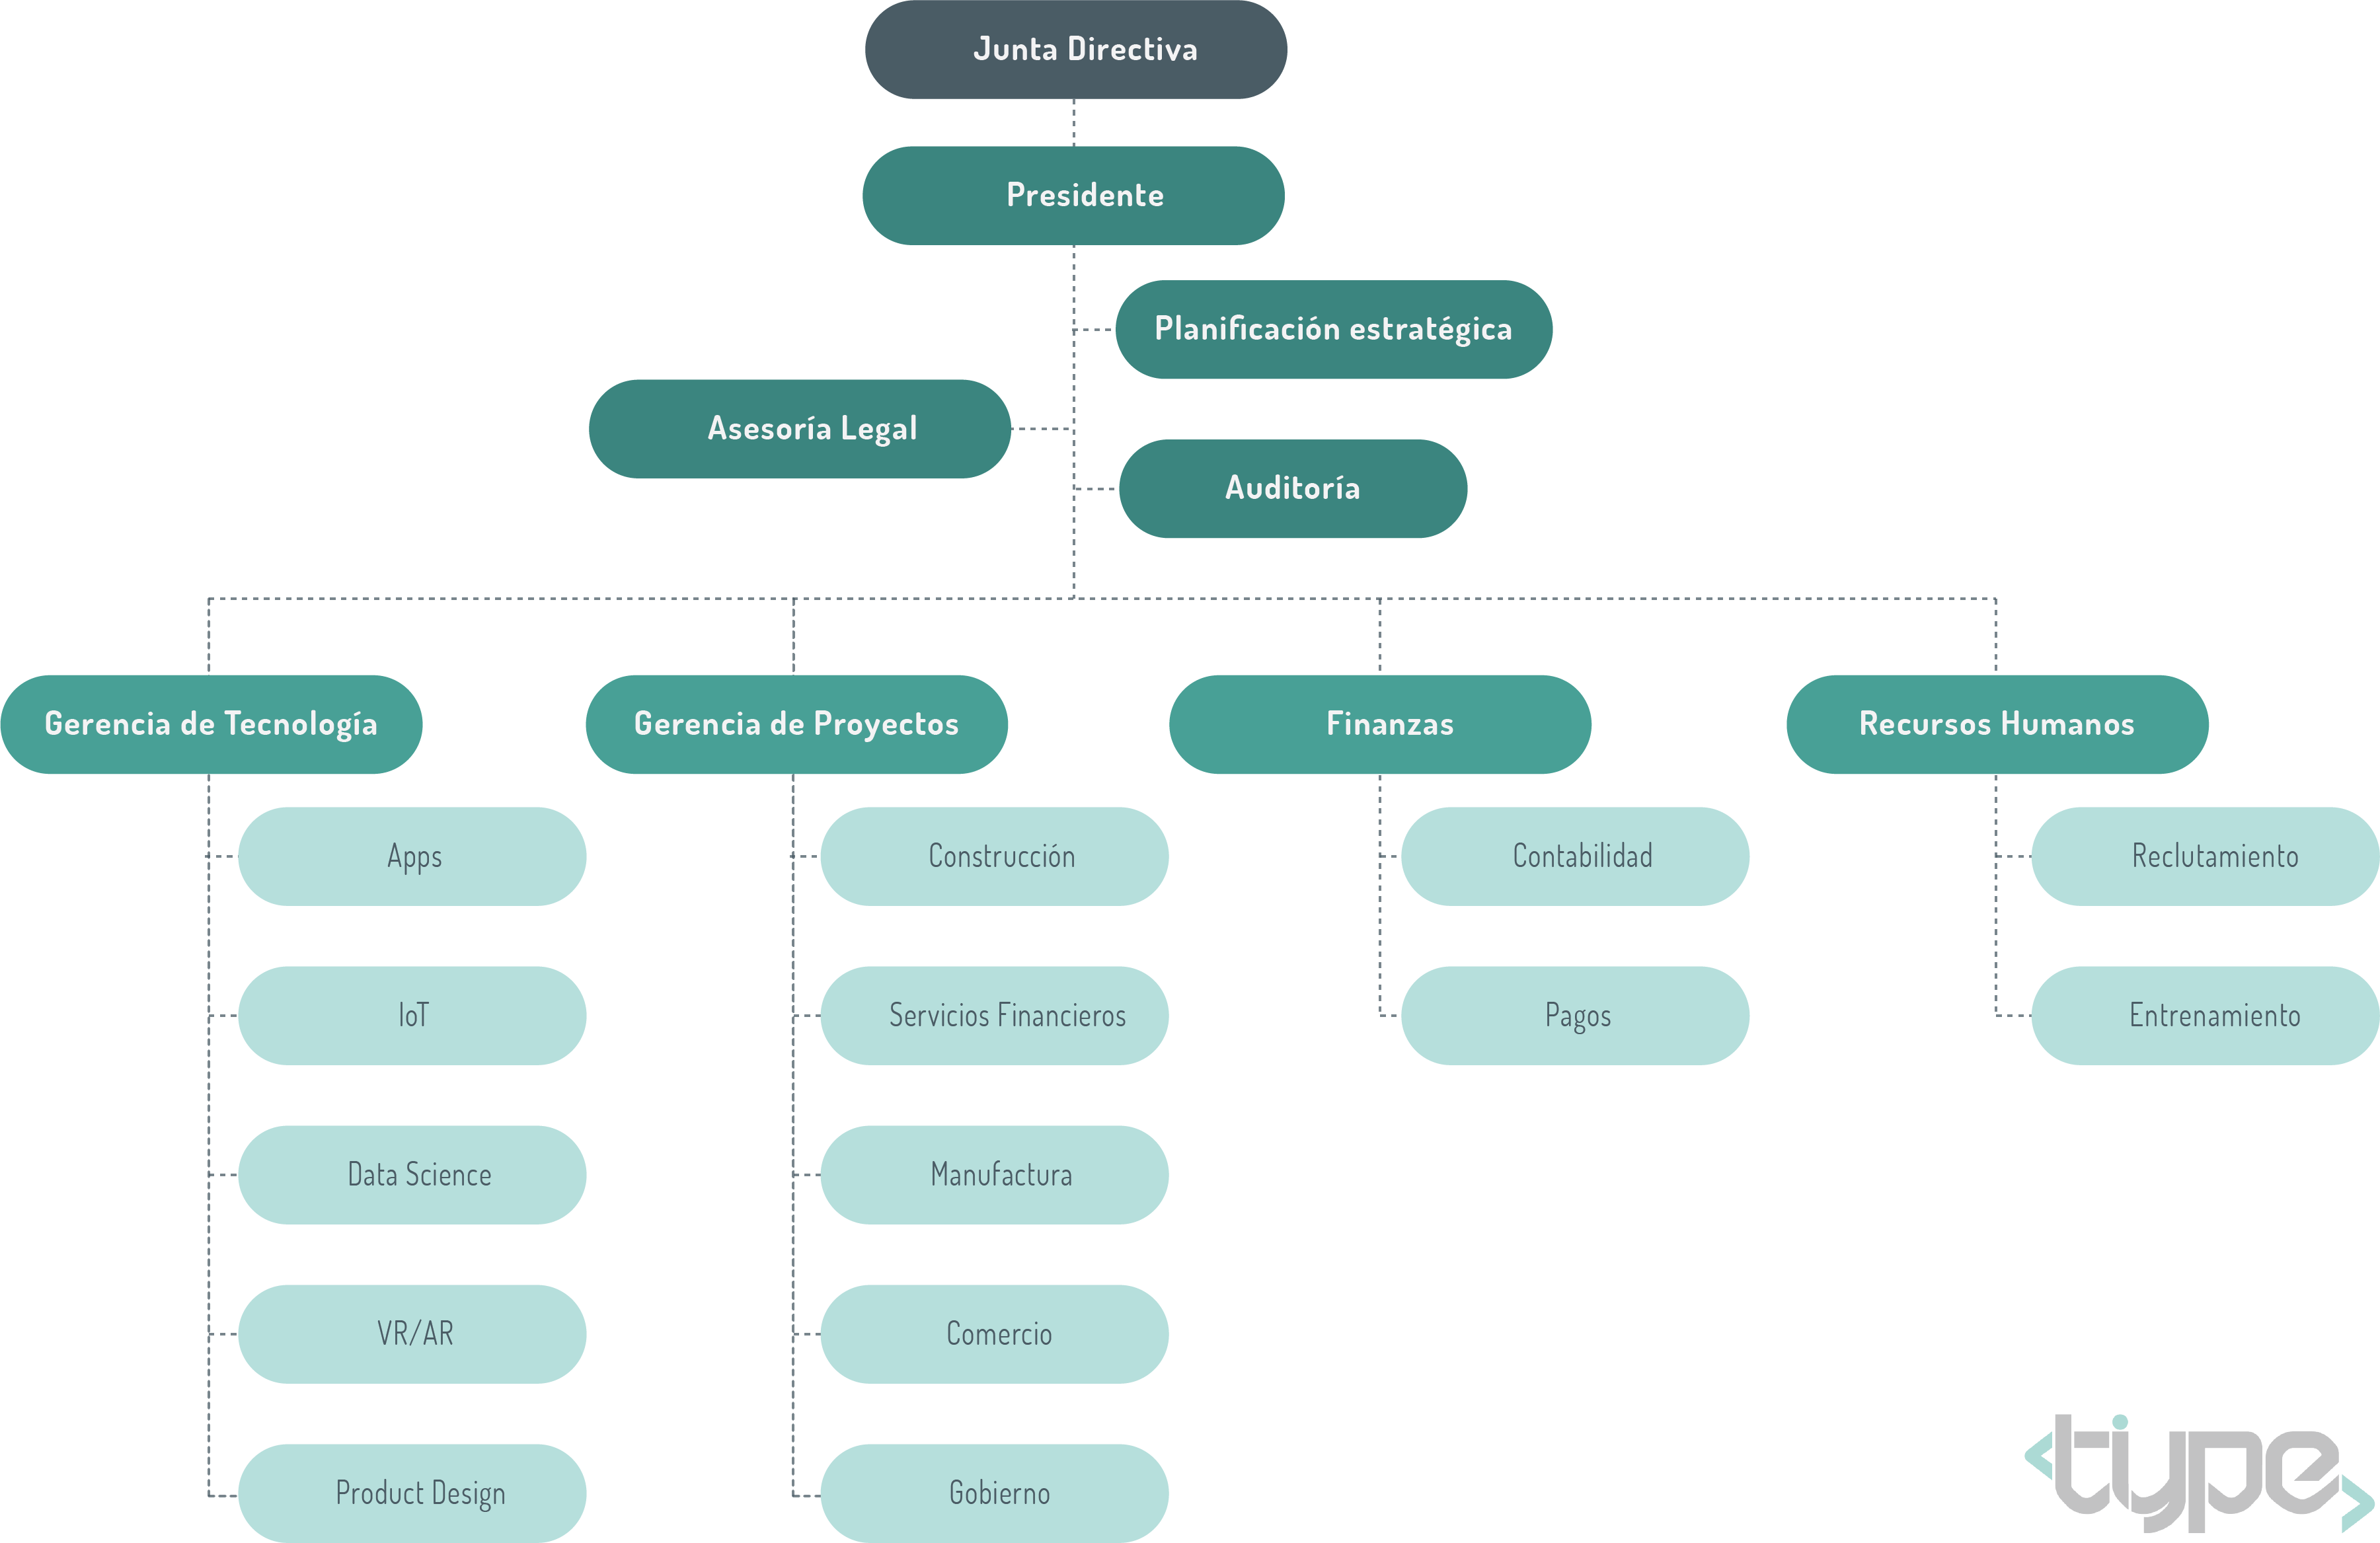
\includegraphics[scale=0.5]
        {Organigrama_type_07082019.png}
    \caption{Estructura de la empresa}
    \label{fig:my_label}
\end{figure}

\newpage
%%%%%%%%%%%%%%%%%%%%%%%%%%%%%%%%%%%%
%%%%%%
%%%%%%         CAPÍTULO II   
%%%%%%
%%%%%%%%%%%%%%%%%%%%%%%%%%%%%%%%%%%   
    \begin{center}
    \setcounter{section}{2}
    \section*{CAPÍTULO II}
    \addcontentsline{toc}{section}{PLANTEAMIENTO DEL PROBLEMA}
    \vspace*{0.5in}
    \textbf{TEMA DE INVESTIGACIÓN}
\end{center}

\subsection{Planteamiento del problema}
%    que es. para que es. y su uso?\\

    Los recursos de generación de energía eléctrica son elementos finitos, sin embargo,  con el transcurso del tiempo la demanda se 
    hace cada vez mayor; en consecuencia se eleva el costo de la energía en proporción al incremento del consumo. La facturación eléctrica
    en distintos países dependen de la oferta y la demanda variando el precio
    en función de las horas en las cuales se genera mayor consumo. Estas variaciones en el costo del servicio generan una 
    oportunidad de ahorro a través de un habito de consumo inteligente.\\
    
    Tradicionalmente las empresas que proveen energía eléctrica calculan los costos con vatímetros analógicos que miden el 
    consumo en una casa, edificio o zona en general. Para obtener la información de este instrumento de medición es 
    requerido que un operario lea la medida implicando costos operativos, además de errores de transcripción o de lectura
    por parte del mismo.\\

    En los últimos años se ha venido desarrollando el Internet de las Cosas (Internet of Things, IoT por sus siglas en inglés),
    el cual es la conexión de dispositivos inteligentes o no a la red internet permitiendo recolectar data y tomar desiciones 
    con la mínima interacción humana. Se desarrollan áreas como inmotica que a través de sensores y dispositivo se automatiza, controla
    y monitorea edificaciones, que integrados a sistemas SCADA costituye todo un sistema.\\

    %El IoT tecnología que se ha venido desarrollando en los últimos años, aprovecha el desarrollo en el área de las 
    %comunicaciones para transmitir información en forma continua e identificada de los instrumentos de medición en un
    %lugar determinado. Dentro de ella surge la inmotica el cual se encarga de la automatización integral de
    %edificaciones, permitiendo el monitoreo y control del mismo.\\
    
    Al emplear herramientas que permitan registrar parámetros de consumo es posible generar un histórico que permitan 
    platear estrategias a corto, mediano y largo plazo para el consumo de la energía.\\

    %Los sistemas SCADA (Supervisory Control And Data Acquisition) son soluciones de software que plantean la adquisición y 
    %control de industrias a distancias. Al desarrollar este tipo de herramienta es posible crear interfaces capaces de 
    %mostrar la información relevante a los usuarios finales permitiendo así establecer planes en base al consumo.\\

    En zonas residenciales se requiere que la empresa que suministra la energía elétrica tenga un historico en tiempo real 
    del comportamiento de consumo de sus usuarios y a su vez que estos usuarios tengan un historico asociado a su consumo 
    que le permita planificar su consumo en función de las horas de menor costo. Para establecer así el consumo inteligente 
    por parte de los usuarios finales, permitendo así reducir costos asociados al costo de la energía.\\
        
    La pasantía se enfoca en el monitoreo de un edificio residencial a través de Mango Automation el cual es una herramienta
    de software que permite desarrollar interfaz para el control y monitorieo de cualquier entorno.

\subsection{Objetivos General}
    Diseñar interfaz SCADA para el 
    monitoreo del consumo energético de un 
    edificio residencial.

\subsection{Objetivos Específicos}
\begin{itemize}
    \item Estudiar funcionalidades y configuración
    del software Mango Automation para el diseño de 
    interfaces.
    \item Identificar variables asociadas al sistema.
    \item Diseñar estructura de las interfaz.
    \item Desarrolarr interfaz asociada al sistema.
\end{itemize}
\newpage
%%%%%%%%%%%%%%%%%%%%%%%%%%%%%%%%%%%%
%%%%%%
%%%%%%         CAPÍTULO III   
%%%%%%
%%%%%%%%%%%%%%%%%%%%%%%%%%%%%%%%%%%   
    \begin{center}
    \setcounter{section}{3}
    \setcounter{subsection}{0}
    \section*{CAPÍTULO III}
    \addcontentsline{toc}{section}{MARCO TEÓRICO}
    \vspace*{0.5in}
    \textbf{MARCO TEÓRICO}
\end{center}

\subsection{SCADA}
    ``Es un concepto que se emplea para realizar un software 
    para ordenadores que permite controlar y supervisar 
    procesos industriales a distancia. Facilita 
    retroalimentación en tiempo real con los 
    dispositivos de campo (sensores y actuadores), y 
    controla el proceso automáticamente. Provee de toda 
    la información que se genera en el proceso 
    productivo (supervisión, control calidad, control de
    producción, almacenamiento de datos, etc.) y 
    permite su gestión e intervención." \textcolor{blue}{\cite{SCADA}}\\

    Este tipo de herramienta estan pensadas para la reducción de costos además de la toma de decisiones automaticas o por 
    desición de los supervisores del proceso. Tradicionalmente son elaborados por expertos en lenguaje de bajo nivel 
    al manejar información principalmente proveniente de sensores, el diagrama basico de un sistema SCADA se representa
    en la Figura \ref{fig:estructura} en donde se plantea un esquema en el cual se adquiere información a través de sensores
    y paneles para el operario cumunicandose con un PLC llevando la información a dispositivos HMI o a interfaz usuario. \\

    Mango Automation ofrece productos de hardware y software para el desarrollo de sistemas SCADA, sin embargo permite que 
    el software se adapte a sistemas ya establecidos realizando la conexión con el software propio del sistema. 
    \begin{figure}[H]
        \centering
        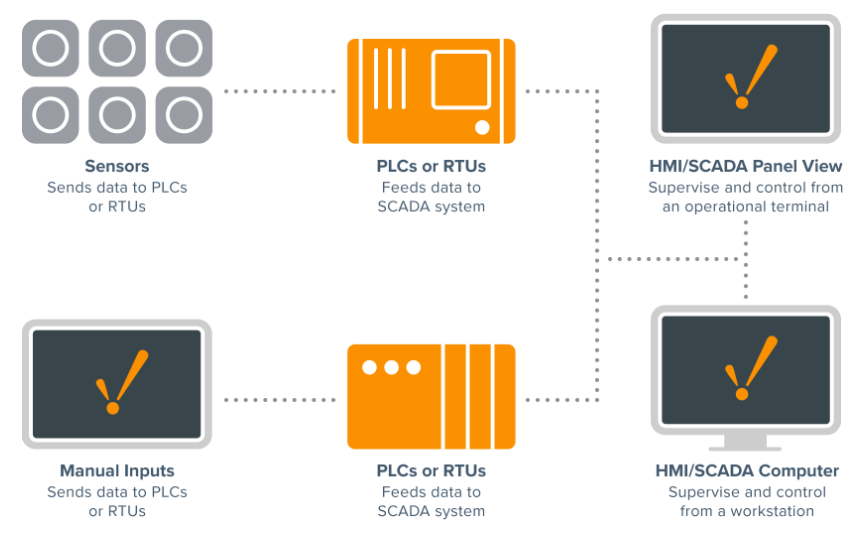
\includegraphics[scale=0.4]
        {EstructuraSCADA.png}
        \caption{Diagrama basico de un sistema SCADA}
    \label{fig:estructura}
    \end{figure}

    

\subsection{Servidor:}
    ``Es un programa informático que procesa una aplicación del lado del servidor, realizando conexiones bidireccionales o unidireccionales y síncronas o asíncronas con el cliente y generando o cediendo una respuesta en cualquier lenguaje o Aplicación del lado del cliente."\textcolor{blue}{\cite{Servidor}}
    
\subsection{Framework:} 
    Es el esquema o estructura que se establece y que se aprovecha para desarrollar y organizar un software determinado.
    ``Un Framework sirve para poder escribir código o desarrollar una aplicación de manera más sencilla. Es algo que permite una mejor organización y control de todo el código elaborado, así como una posible reutilización en el futuro."\textcolor{blue}{\cite{Framework}}
    \\
    Mango Automation implementa AngularJs para el desarrollo de su interfaz como herramienta de desarrollo web permitiendo
    adaptar la interfaz a los requerimientos funcionales y esteticos.
\subsection{Protocolos:} ``En informática y telecomunicación, un protocolo de comunicaciones es un sistema de reglas que permiten que dos o más entidades de un sistema de comunicación se comuniquen entre ellas para transmitir información por medio de cualquier tipo de variación de una magnitud física. Se trata de las reglas o el estándar que define la sintaxis, semántica y sincronización de la comunicación, así como también los posibles métodos de recuperación de errores. Los protocolos pueden ser implementados por hardware, por software, o por una combinación de ambos."\textcolor{blue}{\cite{Protocolo}}
	
\subsection{Escalabilidad:} ``Es un término usado en tecnología para referirse a la propiedad de aumentar la capacidad de trabajo o de tamaño de un sistema sin comprometer el funcionamiento y calidad normales del mismo."\textcolor{blue}{\cite{escalabilidad}}
	
\subsection{Base de datos:} ``Es un conjunto de datos pertenecientes a un mismo contexto y almacenados sistemáticamente para su posterior uso."\textcolor{blue}{\cite{BASE}}
	
%\subsection{LAN:} ``Es una red que conecta los ordenadores en un área relativamente pequeña y predeterminada (como una habitación, un edificio, o un conjunto de edificios)."\textcolor{blue}{\cite{LAN}}
%	
%\subsection{WAN:} ``Red de computadoras que se extiende en una gran franja de territorio, ya sea a través de una ciudad, un país o, incluso, a nivel mundial. "\textcolor{blue}{\cite{WAN}}
	
\subsection{Internet de las cosas (IoT):} ``Agrupación e interconexión de dispositivos y objetos a través de una red (bien sea privada o Internet, la red de redes), dónde todos ellos podrían ser visibles e interaccionar. Respecto al tipo de objetos o dispositivos podrían ser cualquiera, desde sensores y dispositivos mecánicos hasta objetos cotidianos como pueden ser el frigorífico, el calzado o la ropa."\textcolor{blue}{\cite{IOT}}
	
\subsection{Cloud:} ``La computación en la nube son servidores desde Internet encargados de atender las peticiones en cualquier momento. Se puede tener acceso a su información o servicio, mediante una conexión a internet desde cualquier dispositivo móvil o fijo ubicado en cualquier lugar. Sirven a sus usuarios desde varios proveedores de alojamiento repartidos frecuentemente por todo el mundo."\textcolor{blue}{\cite{nube}}
	
\subsection{Interface:} ``Es una conexión entre dos máquinas de cualquier tipo, a las cuales les brinda un soporte para la comunicación a diferentes estratos. Es posible entender la interfaz como un espacio (el lugar donde se desarrolla la interacción y el intercambio)"\textcolor{blue}{\cite{interface}}
    \\

    Se encarga de obtener la información almacenarla y mostrarla de manera mas amigable con el usuario final, idealmente 
    esta debe ser agradable, sencilla además de mostrar data que los usuarios que hacen uso de ella consideren importante.
\subsection{API:} ``Son un conjunto de comandos, funciones y protocolos informáticos que permiten a los desarrolladores crear programas específicos para ciertos sistemas operativos. Las API simplifican en gran medida el trabajo de un creador de programas, ya que no tiene que «escribir» códigos desde cero. Estas permiten al informático usar funciones predefinidas para interactuar con el sistema operativo o con otro programa."\textcolor{blue}{\cite{API}} 
	
\subsection{Mango:} ``Es una aplicación de software multiplataforma basada en web que permite a los usuarios acceder y controlar sensores electrónicos, PLC, controladores, bases de datos o servicios web, a través de múltiples protocolos simultáneamente. Mango proporciona una interfaz con la que se pueden crear y configurar diversas fuentes de datos (data sources), a la vez que proporciona una gestión de accesos a usuarios, registro de datos, alarmas y automatización.\\
	
	Características:
	
	\begin{itemize}
	    \item \textbf{Protocolos integrados:} con BACnet, Modbus, MQTT, SNMP, DNP3, SQL, archivos CSV, HTTP y otros, no es necesario pagar controladores adicionales o herramientas de software. Mango se conectará a todos sus dispositivos y fuentes de datos, integrando todo en una interfaz fácil de usar.
	    
	    \item \textbf{Almacenamiento de datos:} mango es capaz de almacenar billones de valores históricos con un alto rendimiento, mientras utiliza cantidades sorprendentemente pequeñas de espacio en el disco.
	    
	    \item \textbf{Analítica integrada:} mango proporciona varias interfaces web para que los usuarios realicen análisis rápidos y eficientes. Con listas de seguimiento (watch lists) fáciles de configurar y consultas flexibles de datos.
	    
	    \item \textbf{Informes y facturación:} mango proporciona varias interfaces web para que los usuarios realicen análisis rápidos y eficientes. Con listas de seguimiento (watch lists) fáciles de configurar y consultas flexibles de datos.
	    
	    \item \textbf{Horarios y calendarios:} mango cuenta con un planificador que permite programar semanalmente los eventos. También dispone de reglas de excepción que permiten modificar el cronograma predeterminado.
	    
	    \item \textbf{Visualización de datos:}  mango proporciona una plataforma de desarrollo flexible para tableros de control y aplicaciones web/móviles. Con un editor de Drag {\&} Drop, más una vista del código fuente, los usuarios pueden realizar proyectos de manera rápida y eficiente con cualquier nivel de experiencia.
	    
	    \item \textbf{Automatización y alarmas:} mango incluye varios entornos de scripting potentes, que permiten a los usuarios desarrollar cálculos simples o algoritmos de control. Los usuarios pueden configurar varios tipos de alarmas para activar el manejo de eventos o notificaciones, lo que les brinda tranquilidad mientras están ausentes.
	    
	    \item \textbf{APIs}: mango tiene una poderosa arquitectura interna modular (más de 25 módulos de código abierto) que permite a las empresas y desarrolladores crear componentes personalizados. Los módulos pueden ser, desde protocolos hasta aplicaciones completas con sus propios componentes de base de datos."\textcolor{blue}{\cite{MANGO2}}
	    
	\end{itemize}
	
\subsection{MangoES:} ``Es un servidor Linux embebido muy potente basado en ARM con la aplicación completa Mango Enterprise preinstalada. No hay licencias o software adicionales necesarios para operar. Para aplicaciones con menos de 3000 puntos de datos, MangoES reemplaza los costosos servidores con un dispositivo listo para usar. "\textcolor{blue}{\cite{MANGO}}
    
\subsection{Diseño UX/UI:} Es el desarrollo de la experiencia interfaz usuario, donde el esfuerzo se enfoca en hacercar el usuario 
al producto. Siendo como norma perseguir el objetivo del negocio, enmarcarse dentro de las limitaciones tecnicas y satisfacer las
necesidades del usuario siendo este ultimo el pilar del ejercicio.\textcolor{blue}{\cite{AdobeXD}} \textcolor{blue}{\cite{UI}} 

\newpage

%%%%%%%%%%%%%%%%%%%%%%%%%%%%%%%%%%%%
%%%%%%
%%%%%%         CAPÍTULO IV   
%%%%%%
%%%%%%%%%%%%%%%%%%%%%%%%%%%%%%%%%%%   
    \begin{center}
    \setcounter{section}{4}
    \section*{CAPÍTULO IV}
    \addcontentsline{toc}{section}{MARCO METODOLÓGICO}
    \vspace*{0.5in}
    \textbf{MARCO METODOLÓGICO}
\end{center}
\setcounter{subsection}{0}

\subsection{Identificación del sistema}
    Se planteo el monitoreo de un edificio el cual es alimentado con tres fases desde la empresa que suministra energía. 
    A través de un sistema SCADA mostrar variables
    asociadas al consumo generando un histórico que permita obtener valores, en consecuencia obtener
    a partir de este el costo asociado. Las variables del sistema a medir son las siguientes:
    \subsubsection{Variables del sistema}
    \begin{enumerate}
        \item \textbf{Edificio residencial:}

        \begin{itemize}
            \item \textbf{Tensión fase neutro:} Es la tensión suministrada desde el proveedor a la estructura con tres lineas fase
            neutro.
            \item \textbf{Tensión fase neutro promedio:} Es la tensión obtenida al sacar el promedio de las tensiones fase neutro.
            \item \textbf{Tensión fase fase:} Es el valor que se obtiene al medir la tensión entre dos fases.
            \item \textbf{Tensión fase fase prmedio:} Es el valor que se obtiene al obtener el promedio de la tensión fase fase medida anteriormente.
            \item \textbf{Corriente de línea:} Es la corriente suministrada por la central a través de una de las fases, monitorear
            este dato nos puede arrojar que sucede al momento de ocurrir una falla en el circuito.
            \item \textbf{Demanda instantánea activa:} Es la potencia consumida en una de las lineas que provienen desde el 
            distribuidor de energía por norma esta son habitualmente 3 fases generando la potencia activa de la linea uno, dos 
            y tres.
            \item \textbf{Demanda instantánea  activa total:} Se requiere medir y generar un histórico de la potencia instantánea consumida 
            por el conjunto completo, este valor está asociado a la potencia consumida total el cual se define como la suma de 
            la potencia consumida en las 3 fases que alimenta a la infraestructura. 
            \item \textbf{Factor de potencia:} Esta relación nos indica que la corriente consumida se consume e potencia activa 
            manteniendo la corriente en valores calculados.
            \item \textbf{Máxima demanda:} Es la máxima potencia consumida durante un periodo de tiempo.
            \item \textbf{Energía total:} Es la energía consumida referida por defecto a la anterior fecha de pago, con la posibilidad 
            de obtener en función de otro periodo de tiempo definido por el usuario. 
            \item \textbf{Costo total:} Es el costo de la energía consumida desde la anterior fecha de corte.
        \end{itemize}
        Estas variables tienen valores variables instantáneos, es posible generar un historial a través al almacenarlos en una 
        base de datos para mostrarlos en forma grafica.

        \item \textbf{Valores de un apartamento:}
        
        \begin{itemize}
            \item \textbf{Tensión de linea promedio:} Se obtiene al calcular el promedio de las tensiones fase neutro que recibe el inmueble.
            \item \textbf{Demanda activa total:} Es el consumo intantaneo de potencia activa consumida por el inmueble.
            \item \textbf{Energía consumida:} Es la energía consumida por el inmueble durante un periodo de tiempo.
            \item \textbf{Costo acumulado:} Es el costo asociado a la energía consumida.
            \item \textbf{Proxima fecha de pago:} Es la fecha asociada a la proxima fecha de corte de la energía consumida.
            \item \textbf{Estado de conexón:} Valor booleano asociado a la conexión o desconexión del servicio de energía.
        \end{itemize}
    \end{enumerate}
\subsection{Diseño de la estructura de la interfaz}

    En el diseño previo se empleo Adobe XD un software enfocado en el desarrolo UX/UI sin ser requerido el desarrollo del producto para
    poder visualizar la interfaz y la interacción con el usuario. Teniendo en cuenta el tamaño en px disponible en el software de MANGO AUTOMATION
    empleando herramientas de desarrollo en el buscador Chrome obteniendo de allí los colores bases y los tamaños estandares para el dieño.\\

    Se diseñan las siguientes insterfaces:\\
    \begin{itemize}

        \item \textbf{Overview:} Se plantea una interfaz (Figura \ref{figInterfazOverview}) en la cual se tiene la ubicación geografica de los edificios
        en monitoreo donde se presenta la información del nombre del edificio, demanda instantánea, Energía total acumulada y el costo total asociado al 
        consumo de energía consumida. Pensando en el monitoreo de distintos edificios permitiendo hacer uso de la plataforma en la administración de
        distintos condominios por parte de una empresa.

        \begin{figure}[H]
            \centering
                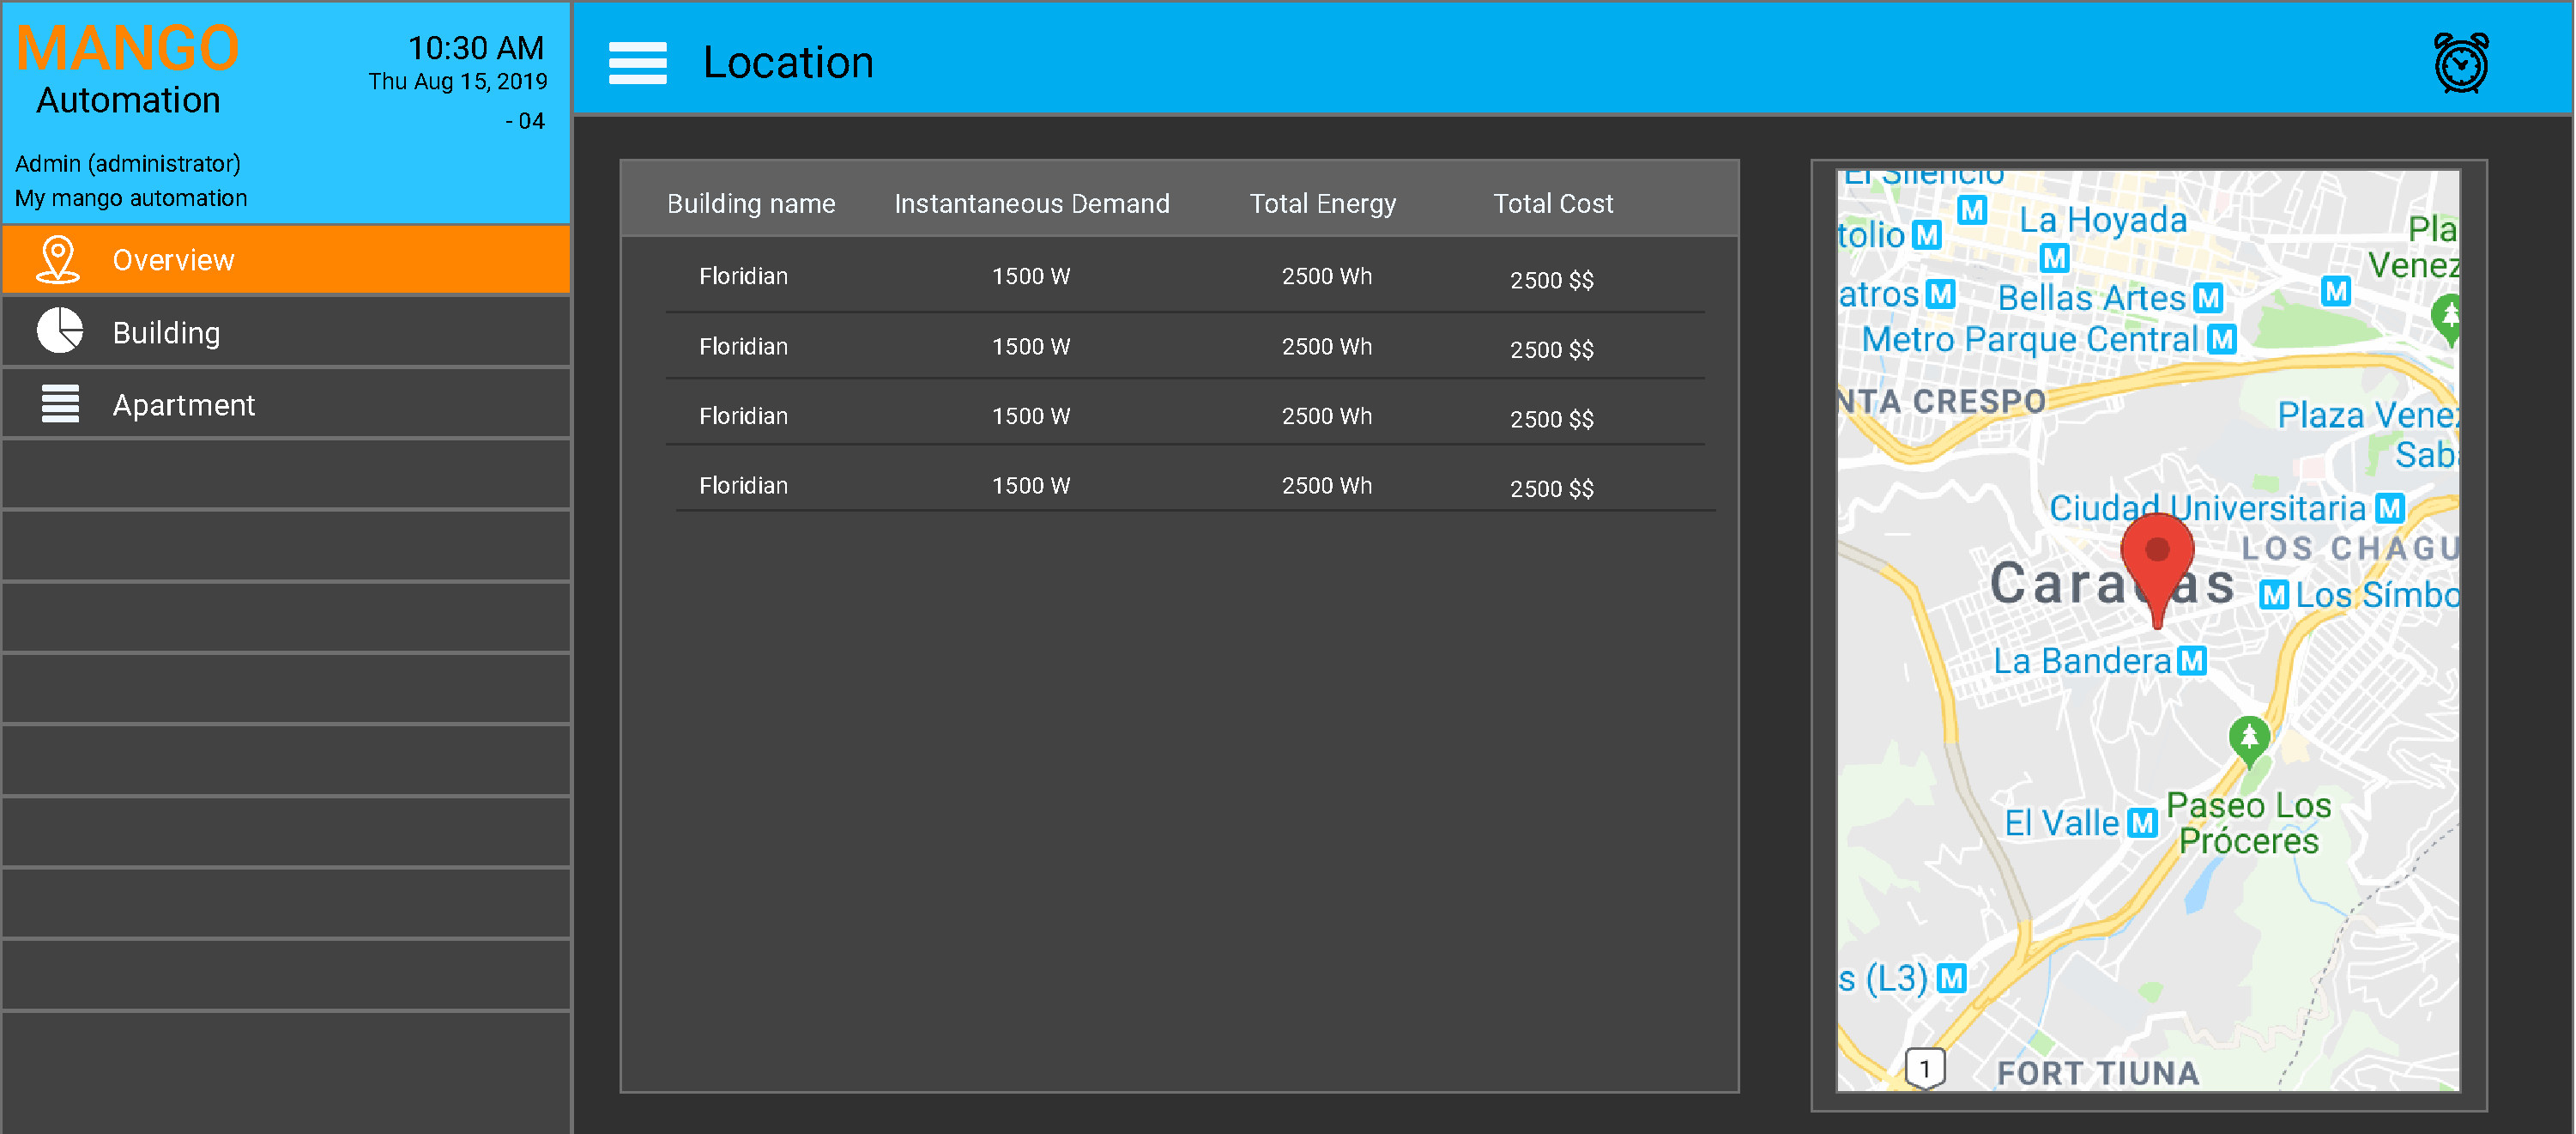
\includegraphics[scale=0.2]
                {overview.pdf}
            \caption{Interfaz overview}
            \label{figInterfazOverview}
        \end{figure} 
        
        \item \textbf{Building:} Se plantea una interfaz (Figura \ref{figInterfazBuilding}) donde se hace enfoque a cuatro variables Demanda Instantánea, Demanda Máxima, Energía Total y 
        Costo total enfocándose en parametros claves de costo y consumo.
        
        \begin{figure}[H]
            \centering
                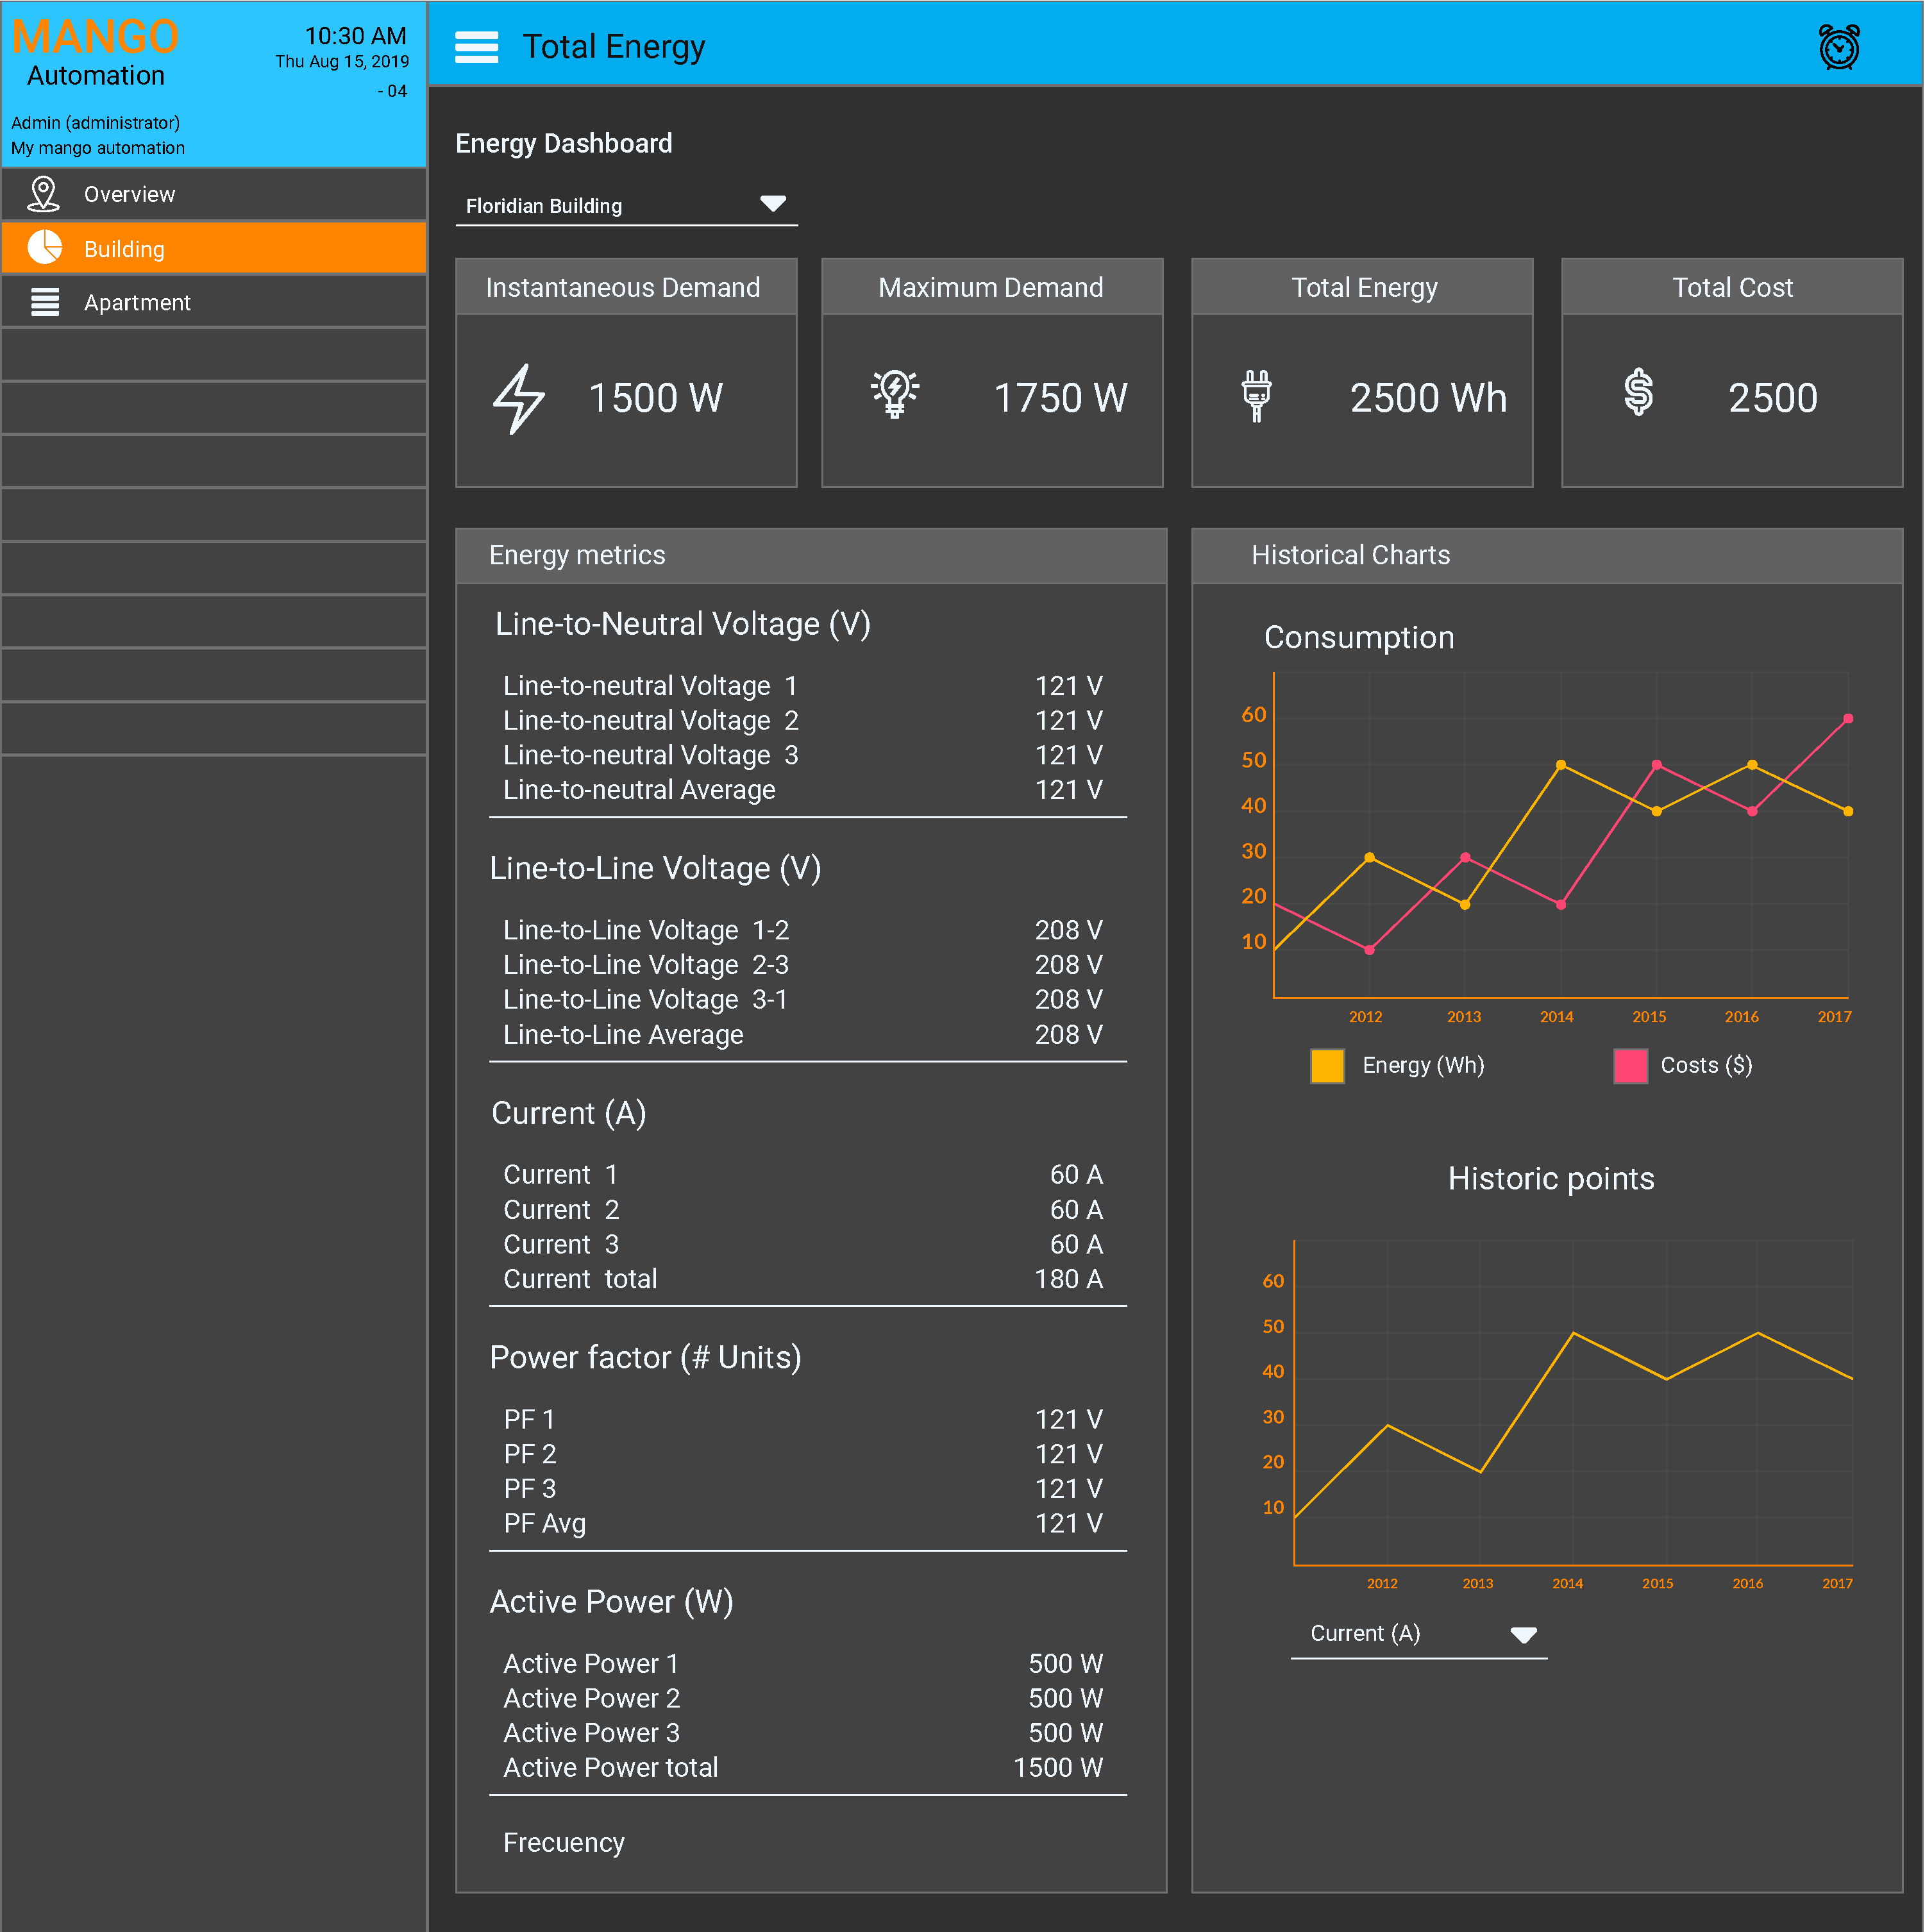
\includegraphics[scale=0.2]
                {building.pdf}
            \caption{Interfaz building}
            \label{figInterfazBuilding}
        \end{figure}

        Se diseñan dos bloques de información un primer asociado a las metricas instantánea con valores que permiten el monitoreo con valores de tensión, corriente,
        potencia, factor de potencia y frecuencia de la red y un segundo de bloque en donde se plantean graficas de la data obtenida a través del tiempo.
        Se estructura de tal manera que a primera vista con fines de administración financiera se obtiene la data importante para tal actividad, en caso de requerir
        monitoreo tecnico se presenta la información requerida para una rapida toma de decisiones o un analísis del sistema a través del tiempo.
 
        \item \textbf{Apartment:} Se plantea una interfaz (Figura \ref{figInterfazApartment}) el cual esta pensado para el usuario final y datos requeridos
        para estudios tecnicos por parte de un tecnico. Se presentan datos a la energía consumida, el costo asociado, la próxima fecha de pago, 
        y pagos retrasados, valores económicos importantes para el usuario que paga la cuenta de energía electrica además de valores que permitan 
        realizar estudios en caso de ser requeridos.

        \begin{figure}[H]
            \centering
                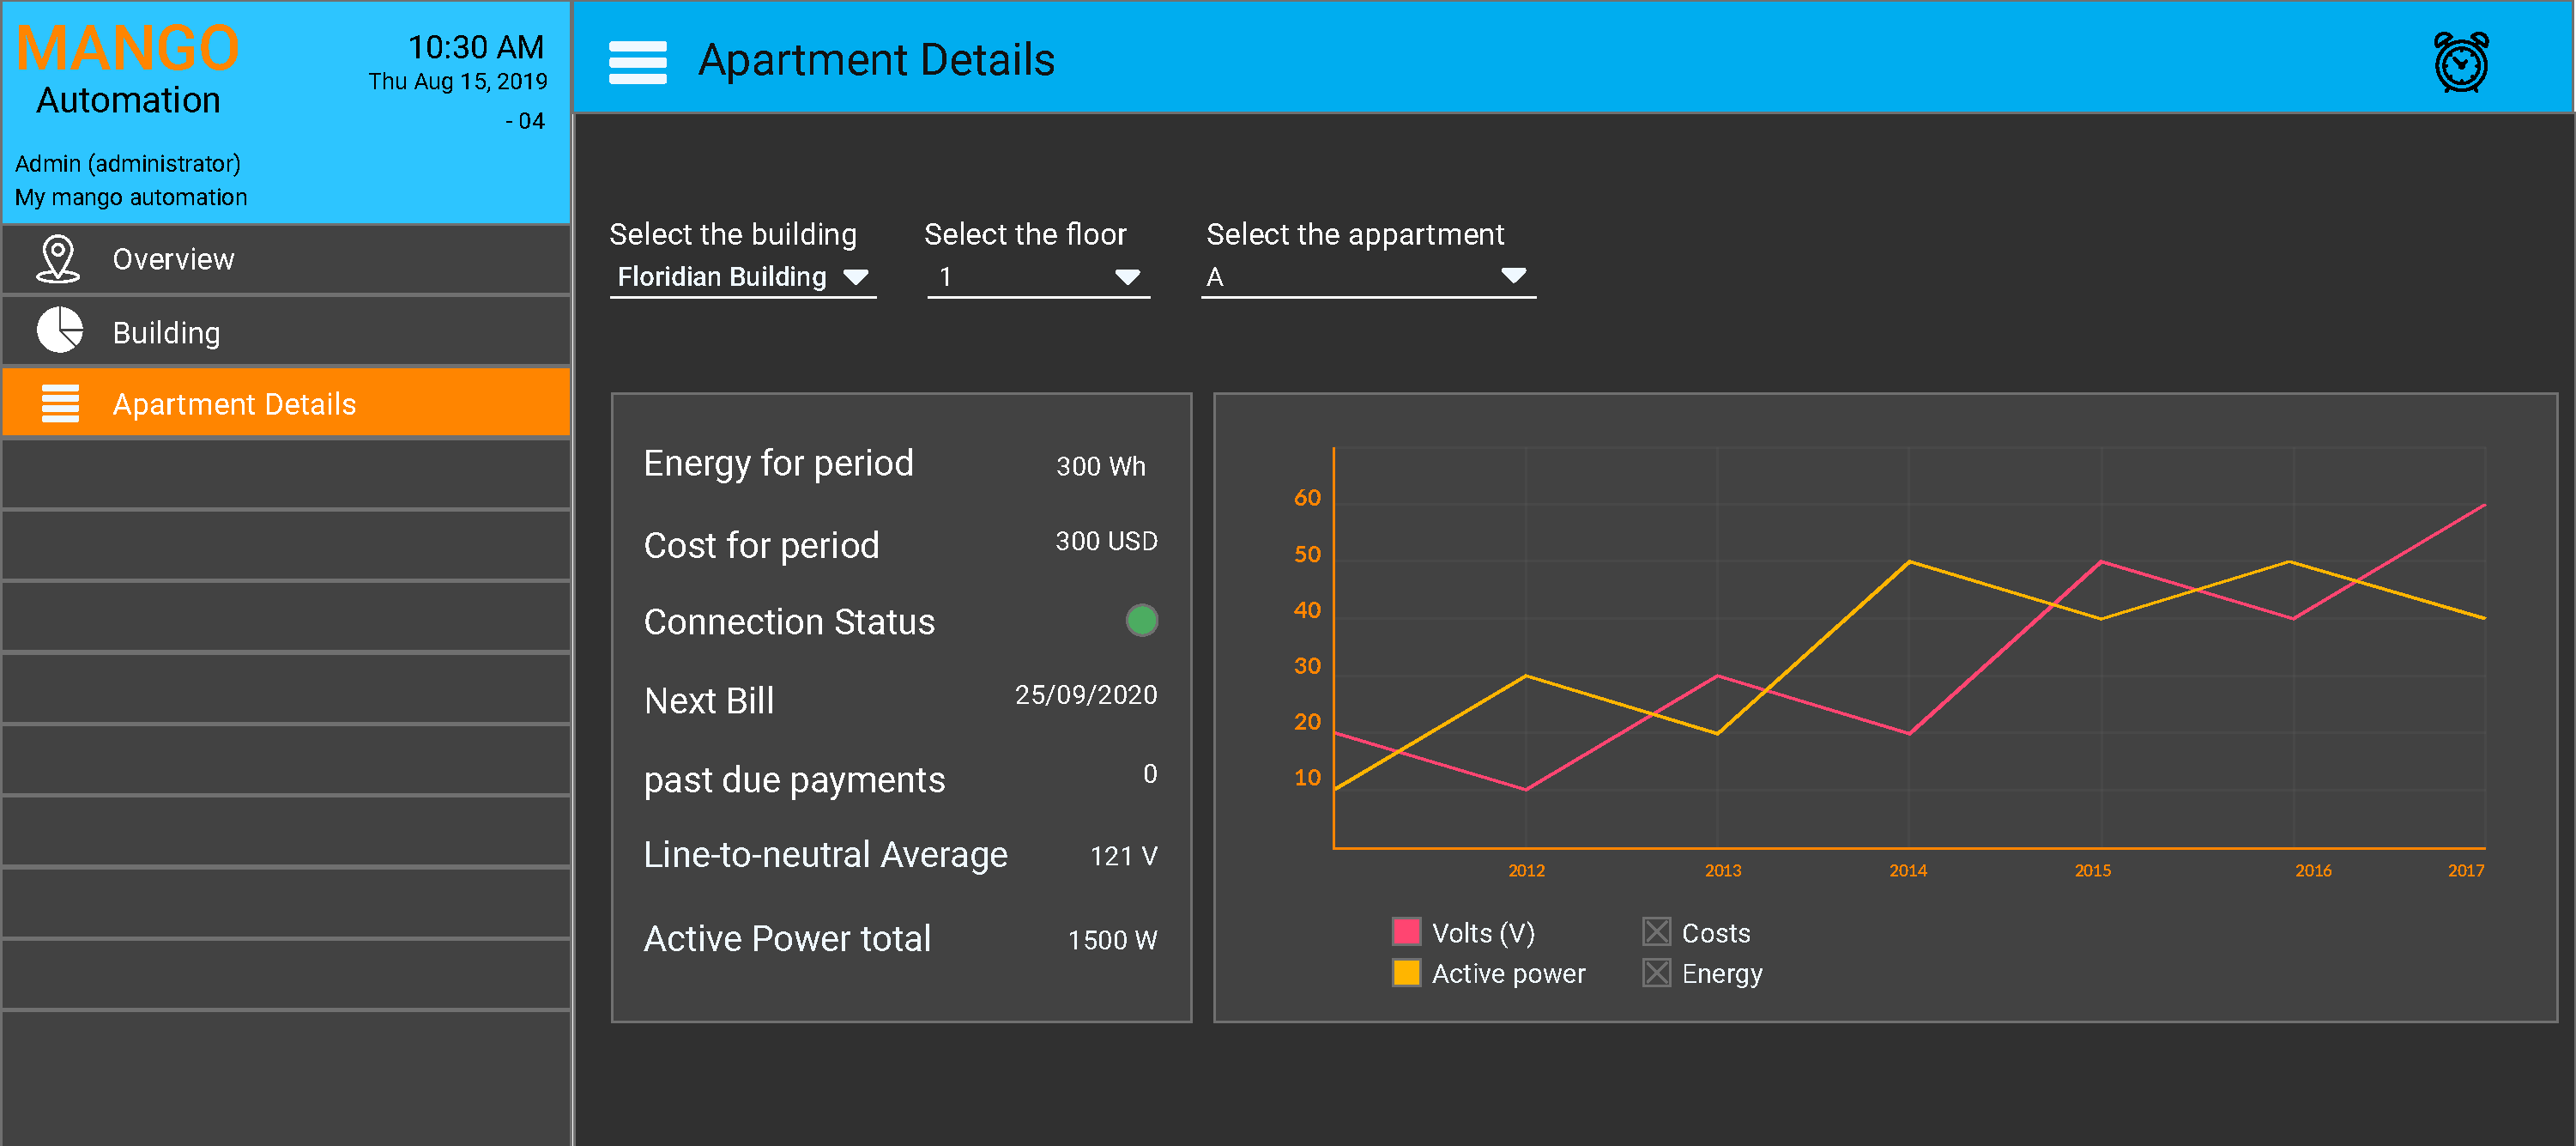
\includegraphics[scale=0.2]
                {apartment.pdf}
            \caption{Interfaz apartament}
            \label{figInterfazApartment}
        \end{figure}
    \end{itemize}
\subsection{Definición de Variables en plataforma de Mango AUTOMATION}
    La plataforma permite definir variables con el protocolo de comunicación a establecer, en nuetro caso se emplean Virtual Data Point 
    y meta Data source, la primera para generar de forma aleatoria da
\subsection{Desarrollo de la interfaz}
    
\newpage
%%%%%%%%%%%%%%%%%%%%%%%%%%%%%%%%%%%%
%%%%%%
%%%%%%         CAPÍTULO V   
%%%%%%
%%%%%%%%%%%%%%%%%%%%%%%%%%%%%%%%%%%   
    \begin{center}
    \section*{CAPÍTULO V}
    \addcontentsline{toc}{section}{PROCESO DE ANÁLISIS Y CÁLCULO}
    \vspace*{0.5in}
    \textbf{PROCESO DE ANÁLISIS Y CÁLCULO}
\end{center}

\newpage
%%%%%%%%%%%%%%%%%%%%%%%%%%%%%%%%%%%%
%%%%%%
%%%%%%         CAPÍTULO VI   
%%%%%%
%%%%%%%%%%%%%%%%%%%%%%%%%%%%%%%%%%%   
    \begin{center}
    \section*{CAPÍTULO VI}
    \addcontentsline{toc}{section}{RESULTADOS}
    \vspace*{0.5in}
    \textbf{RESULTADOS}
\end{center}

\newpage
%%%%%%%%%%%%%%%%%%%%%%%%%%%%%%%%%%%%
%%%%%%
%%%%%%         CAPÍTULO VII   
%%%%%%
%%%%%%%%%%%%%%%%%%%%%%%%%%%%%%%%%%%   
    \begin{center}
    \section*{CAPÍTULO VII}
    \addcontentsline{toc}{section}{ANÁLISIS DE RESULTADOS}
    \vspace*{0.5in}
    \textbf{ANÁLISIS DE RESULTADOS}
\end{center}

\newpage
%%%%%%%%%%%%%%%%%%%%%%%%%%%%%%%%%%%%
%%%%%%
%%%%%%         CAPÍTULO VIII   
%%%%%%
%%%%%%%%%%%%%%%%%%%%%%%%%%%%%%%%%%%   
    \begin{center}
    \section*{CAPÍTULO VIII}
    \addcontentsline{toc}{section}{CONCLUSIONES}
    \vspace*{0.5in}
    \textbf{CONCLUSIONES}
\end{center}

\newpage
%%%%%%%%%%%%%%%%%%%%%%%%%%%%%%%%%%%%
%%%%%%
%%%%%%         CAPÍTULO IX  
%%%%%%
%%%%%%%%%%%%%%%%%%%%%%%%%%%%%%%%%%%   
    \begin{center}
    \section*{CAPÍTULO IX}
    \addcontentsline{toc}{section}{RECOMENDACIONES}
    \vspace*{0.5in}
    \textbf{RECOMENDACIONES}
\end{center}

\newpage
%%%%%%%%%%%%%%%%%%%%%%%%%%%%%%%%%%%%
%%%%%%
%%%%%%         CAPÍTULO X   
%%%%%%
%%%%%%%%%%%%%%%%%%%%%%%%%%%%%%%%%%%   
    \begin{center}
    \section*{CAPÍTULO X}
    \addcontentsline{toc}{section}{BIBLIOGRAFÍA}
	\vspace*{0.5in}
	\renewcommand{\refname}{BIBLIOGRAFÍA}
\end{center}

\begin{thebibliography}{10}

	\bibitem {SCADA} "SCADA", Es.wikipedia.org, 2019. [Online]. Available: https://es.wikipedia.org/wiki/SCADA. [Accessed: 07- Aug- 2019].

	\bibitem {MANGO}"MANGOES", Static1.squarespace.com, 2019. [Online]. Available: https://static1.squarespace.com/static/587820255016e182d0570766/t/5ab301b45
	
	62fa79e4d50d97d/1521680822626/Mango+Spec+-+Spanish.pdf.
	
	[Accessed: 07- Aug- 2019].{MANGO} MANGOES. 2019, p. 1.
	
	\bibitem{Servidor}"Servidor web", Es.wikipedia.org, 2019. [Online]. Available: https://es.wikipedia.org/wiki/Servidor\_web. [Accessed: 07- Aug- 2019].
	
	\bibitem{LAN} "¿Qué es una red LAN? - Definición de LAN", Masadelante.com, 2019. [Online]. Available: https://www.masadelante.com/faqs/lan. [Accessed: 07- Aug- 2019].
	
	\bibitem{WAN} "Definición de WAN — Definicion.de", Definición.de, 2019. [Online]. Available: https://definicion.de/wan/. [Accessed: 07- Aug- 2019].
	
	\bibitem{BASE}"Base de datos", Es.wikipedia.org, 2019. [Online]. Available: https://es.wikipedia.org/wiki/Base\_de\_datos. [Accessed: 07- Aug- 2019].
	
	\bibitem{Framework}"¿Qué es un Framework y para que sirve? - Neo Wiki | NeoAttack", Neoattack, 2019. [Online]. Available: https://neoattack.com/neowiki/framework/. [Accessed: 07- Aug- 2019].
	
	\bibitem{IOT} "¿Qué es IoT (Internet Of Things)?", Deloitte Spain, 2019. [Online]. Available: https://www2.deloitte.com/es/es/pages/technology/articles/IoT-internet-of-things.html. [Accessed: 07- Aug- 2019].
	
	\bibitem{Protocolo}"Protocolo de comunicaciones", Es.wikipedia.org, 2019. [Online]. Available: https://es.wikipedia.org/wiki/Protocolo\_de\_comunicaciones[Accessed: 07- Aug- 2019].
	
	\bibitem{escalabilidad}"¿A qué se refieren con eso de escalabilidad?", aboutespanol, 2019. [Online]. Available: https://www.aboutespanol.com/que-es-escalabilidad-157635. [Accessed: 07- Aug- 2019].
	
	\bibitem{nube}"Computación en la nube", Es.wikipedia.org, 2019. [Online]. Available: https://es.wikipedia.org/wiki/Computaci\%C3\%B3n\_en\_la\_nube. [Accessed: 07- Aug- 2019].
	
	\bibitem{interface} "Definición de interfaz — Definicion.de", Definición.de, 2019. [Online]. Available: https://definicion.de/interfaz/. [Accessed: 07- Aug- 2019].
	
	\bibitem{API} "¿Qué es una API y para qué sirve?", abc, 2019. [Online]. Available: https://www.abc.es/tecnologia/consultorio/20150216/abci--201502132105.html. [Accessed: 07- Aug- 2019].
	
	\bibitem{MANGO2} "MANGO AUTOMATION", Infiniteautomation.squarespace.com, 2019. [Online]. Available: https://infiniteautomation.squarespace.com/s/Mango-Automation-Brochure-Spanish.pdf. [Accessed: 07- Aug- 2019].
	
	\bibitem{AdobeXD} Villalobos, M. (2019). "Experiencia de Usuario: ¿Qué es y cómo convertirse en UX Designer?". Retrieved 24 September 2019, from https://medium.com/repensareducativo/experiencia-de-usuario-qu\%C3\%A9-es-y-c\%C3\%B3mo-convertirse-en-ux-designer-ec27d3844c97

	\bibitem{UI} Cantú, A. (2019). "Qué es: UX y UI" | Andrea Cantú. Retrieved 24 September 2019, from https://blog.acantu.com/que-es-ux-y-ui/
\end{thebibliography}
\newpage
%%%%%%%%%%%%%%%%%%%%%%%%%%%%%%%%%%%%
%%%%%%
%%%%%%         Apendice  
%%%%%%
%%%%%%%%%%%%%%%%%%%%%%%%%%%%%%%%%%%   
\begin{center}
    \section*{APÉNDICE}
    \addcontentsline{toc}{section}{APÉNDICE}
\end{center}


\end{document}